\newpage
\section{Original Requirements Document}
\def\RDtitle{Computer Science Senior Software Engineering Project (CS462)}
\def\RDversion{2.0}
\def\RDterm{Winter 2017}

	\centering
	\vspace{\fill}

	{\Huge\bfseries Original Requirements Document\par}
	\vspace{0.5cm}
	{\Large\itshape \RDtitle\par}
	\vspace{0.5cm}
	{\Large\itshape \RDterm\par}
	
	\vspace{\fill}
	
	\begin{abstract}
	We are working with Rockwell Collins to explore potential technological innovations relating to their Head-Up Display (HUD) systems that present critical flight information to pilots. Our primary objective is to improve Rockwell Collins current HUD systems by reducing the cost and time required to precisely align flight information to the HUD. To meet our objective we will look into using a new alignment methodology in conjunction with the current HUD system as a proof of concept. The product being developed is a demonstration system that looks to include a MEMS IRU mounted onto the HUD and a new alignment algorithm that utilizes this additional sensor to determine accurate HUD alignment. This document will introduce the specific details of the demonstration system and describe the requirements for the development of the product.
	\end{abstract}
	
	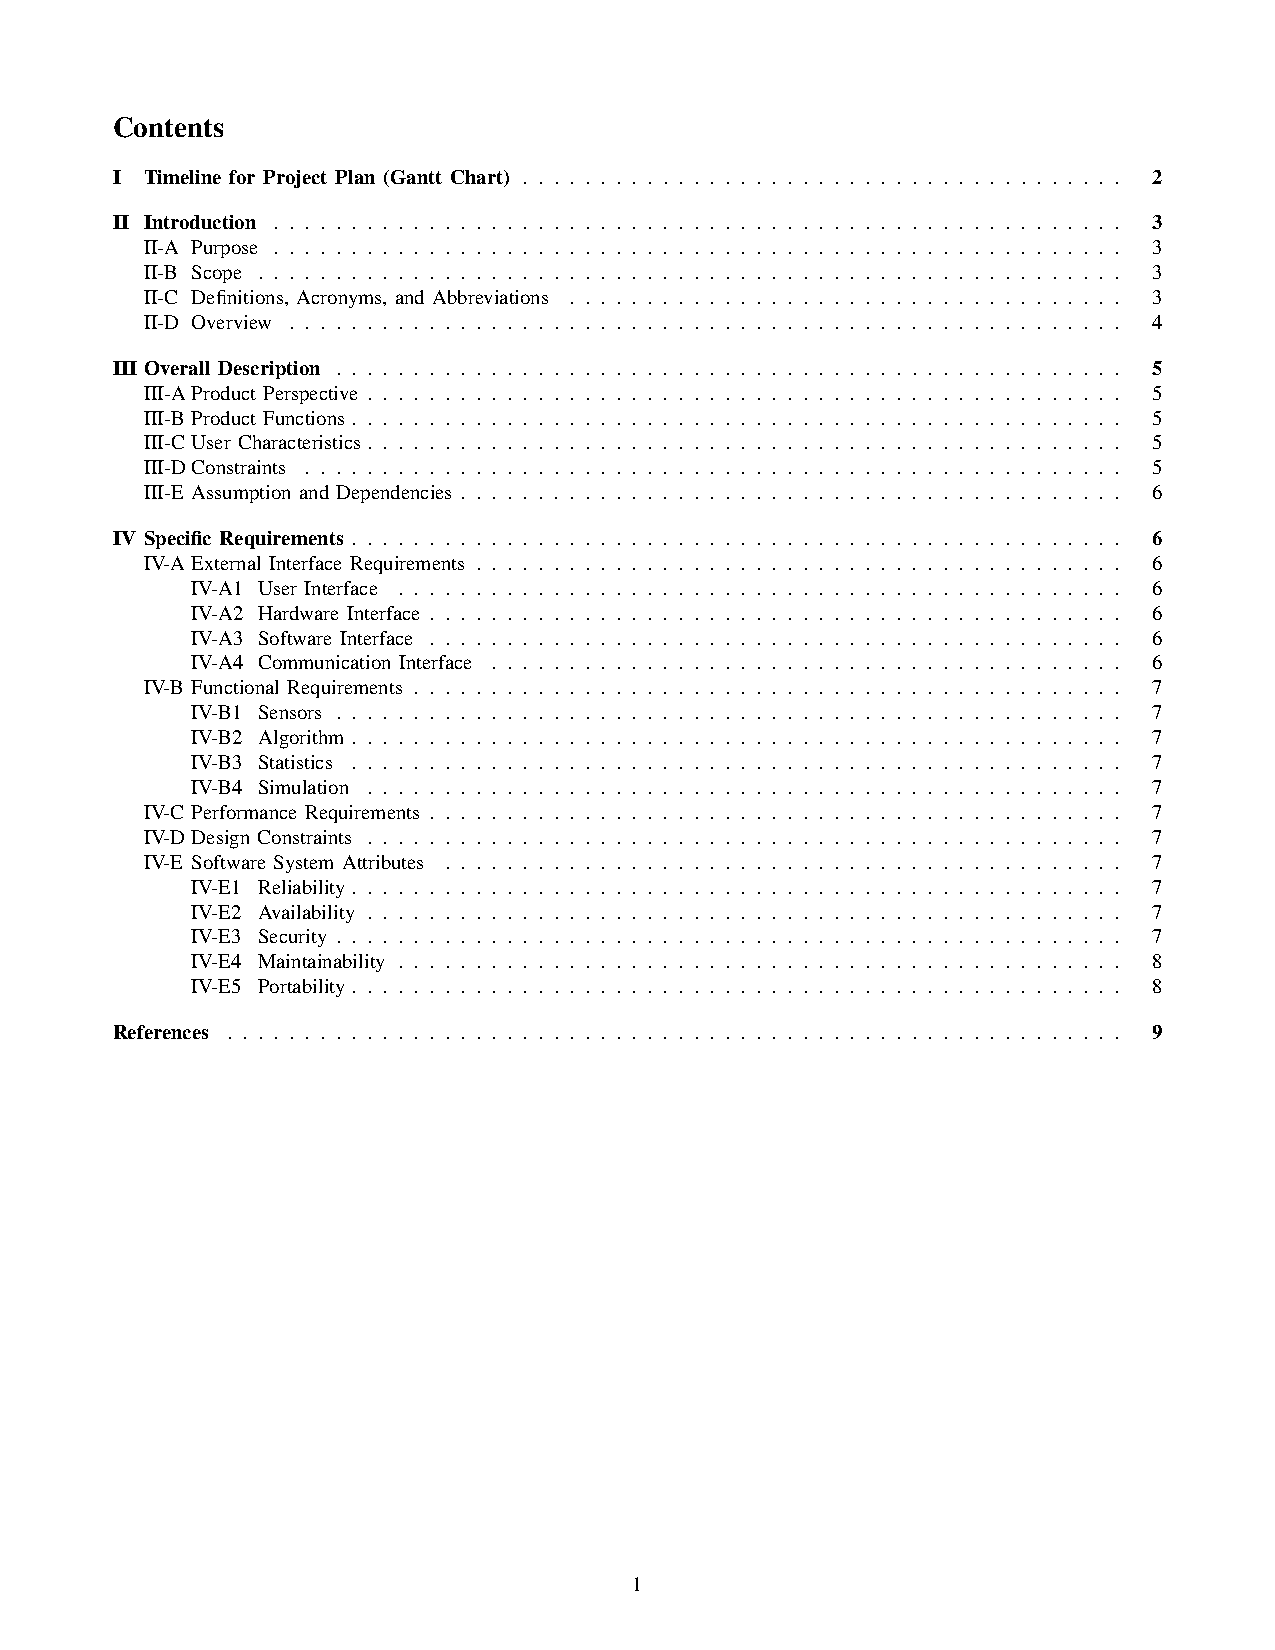
\includepdf[pages=-]{pdf/req_doc.pdf}